% !TEX TS-program = pdflatex
% !TEX encoding = UTF-8 Unicode

\documentclass[11pt]{article} % use larger type; default would be 10pt

\usepackage[utf8]{inputenc} % set input encoding (not needed with XeLaTeX)

%%% PAGE DIMENSIONS
\usepackage{geometry} % to change the page dimensions
\geometry{a4paper}
%%% PACKAGES
\usepackage{graphicx} % support the \includegraphics command and options
\usepackage{booktabs} % for much better looking tables
\usepackage{array} % for better arrays (eg matrices) in maths
\usepackage{paralist} % very flexible & customisable lists (eg. enumerate/itemize, etc.)
\usepackage{verbatim} % adds environment for commenting out blocks of text & for better verbatim
\usepackage{subfig} % make it possible to include more than one captioned figure/table in a single float
\usepackage{amssymb}
\usepackage{mathtools}
\usepackage{algorithm}
\usepackage{algpseudocode}
\usepackage{graphicx}
\usepackage{makecell}
\usepackage{url}
\graphicspath{ {./res/} }

%%% HEADERS & FOOTERS
\usepackage{fancyhdr}
\pagestyle{fancy} % options: empty , plain , fancy
\renewcommand{\headrulewidth}{0pt} % customise the layout...
\lhead{}\chead{}\rhead{}
\lfoot{}\cfoot{\thepage}\rfoot{}

%%% SECTION TITLE APPEARANCE
\usepackage{sectsty}
\allsectionsfont{\sffamily\mdseries\upshape}

%%% ToC (table of contents) APPEARANCE
\usepackage[nottoc,notlof,notlot]{tocbibind} % Put the bibliography in the ToC
\usepackage[titles,subfigure]{tocloft} % Alter the style of the Table of Contents
\renewcommand{\cftsecfont}{\rmfamily\mdseries\upshape}
\renewcommand{\cftsecpagefont}{\rmfamily\mdseries\upshape} % No bold!

\DeclarePairedDelimiter\abs{\lvert}{\rvert}%
\DeclarePairedDelimiter\floor{\lfloor}{\rfloor}%
\DeclarePairedDelimiter\fract{fract(}{)}

\renewcommand{\listfigurename}{Index des illustrations}

% Custom ParFor (parallel for) command in algorithms
\algblock{ParFor}{EndParFor}
\algnewcommand\algorithmicparfor{\textbf{parfor}}
\algnewcommand\algorithmicpardo{\textbf{do}}
\algnewcommand\algorithmicendparfor{\textbf{end\ parfor}}
\algrenewtext{ParFor}[1]{\algorithmicparfor\ #1\ \algorithmicpardo}
\algrenewtext{EndParFor}{\algorithmicendparfor}

%%% END Article customizations


\title{Rapport de projet\\Génération de terrain et affichage 3D}
\author{Van Hollebeke Joshua\\Calais Albin}
\begin{document}
\maketitle

\section{Contexte}

%% TODO intro 

Notre projet consiste à créer un générateur de terrain et à afficher ce terrain d'une manière réaliste. Pour cela nous développerons des algorithmes de génération, des interfaces de dialogue avec le gpu et des systèmes d'affichage très complexes.

Ce projet sera écrit en C++ pour permettre une gestion avancé de la mémoire et des performances, il facilitera aussi l'utilisation de l'api graphique OpenGL.
Nous utiliserons plusieurs algorithmes connus et d'autres tirés de papiers de recherche, nous en concevrons et adapterons certains car notre cas d'utilisation est assez particulier.

La plupart des systèmes que nous construirons existent déjà mais nous essayerons d'y apporter des améliorations.

\paragraph{}
Pour les systèmes existants, nous utiliserons la terminologie anglaise plutôt que française.

\section{Conception et gestion de projet}

D'un point de vue global notre projet est assez simple, il se compose seulement de deux modules de haut niveau qui utilisent chacun plusieurs modules de plus bas niveau.

%% TODO uml [Generation] + [Affichage->OpenGL]

\subsection{Conception structurelle}

Nous avons passé un certain temps en amont sur la concéption globale de l'application. Elle ressemble à ce qu'on trouverait dans un \textit{Game Engine} moderne du type Unity ou Unreal Engine. Il existe une unique \textit{scène} - un monde - qui contient des objets qui sont affichés et mis à jours régulièrement.

%% TODO uml [Generation]->[scene]->player->camera  ->terrain->chunks  ->...   ->[Renderer]

La scène est construite une seule fois et le joueur y existe et peut s'y balader. La scène est globalement statique, les seuls objets qui se déplacent sont le joueur et le soleil, le reste est figé en place mais peut être animé d'autres manières.

\subsection{Tests, sandbox}

Ce genre de projet est très peu propice aux tests, pour s'assurer du bon fonctionnement global de l'application nous nous baserons sur des tests d'intégration seulement. Pour chaque fonctionnalité nous créerons une scène qui présentera seulement la fonctionnalité en question, de cette manière il sera très simple de vérifier le bon fonctionnement de chaque partie du système.

En plus de ces scènes de test, nous créérons des scènes \textit{sandbox} qui intégreront toutes les fonctionnalités et serviront de démonstration techniques des résultats que nous obtiendrons.

%% TODO liste des scènes <-> fonctionnalités

\section{Génération de terrain}

Pour générer notre terrain, il nous faut d'abord lister les contraintes que nous nous fixons - et celles que nous ignorons - ; nous voulons :
\begin{itemize}
	\item{un grand terrain}
	\item{sans répétitions}
	\item{assez détaillé}
	\item{dont la hauteur change}
\end{itemize}

Nous nous restreindrons à une seule valeur de hauteur par position dans le plan, donc pas de grottes ou de surplomb. Les algorithmes classiques qui correspondent à ces critères consistent à créer une \textit{carte de hauteur} (\textit{heightmap}) et à placer des points sur une grille dont les hauteurs correspondent à celles de la carte. Il suffit ensuite de relier ces points pour avoir un terrain convainquant comme illustré par la figure \ref{fig:wireframe_terrain}.

\begin{figure}[h]
	\centering
	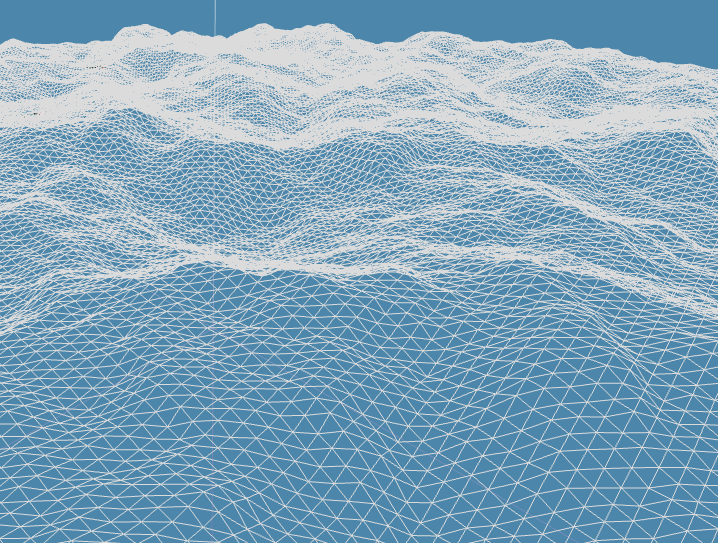
\includegraphics[scale=.49]{terrain_wireframe}
	\caption{Un squelette de terrain fait à partir d'une grille sculptée} %% TODO trouver le bon mot pour "displaced" plutot que sculptée
	\label{fig:wireframe_terrain}
\end{figure}

Il existent d'autres méthodes pour faire ce genre de terrain (cubemarching, raymarching avec génération dynamique...) qui permettent de faire plus mais qui sont beaucoup plus gourmandes en performances et en complexité. Dans notre cas une heightmap est beaucoup plus adaptée.

\subsection{Bruit de Perlin}

Pour créer la heightmap il nous faut ce qu'on appelle un \textit{bruit}, une fonction dont le domaine de définition est le plan $xz$ et le domaine de valeurs est $\mathbb{R}$. Cette fonction doit être pseudo-aléatoire mais deterministe. La plus simple est le \textit{white noise} qui est "complètement aléatoire"\footnote{On utilisera le générateur de nombre pseudo-aléatoires de C++ pour attribuer une valeur à chaque point du plan $\mathbb{Z}^2$.}. On s'interessera plutôt aux fonctions de bruit continues sur $\mathbb{R}^2$.

\begin{figure}[h]
	\centering
	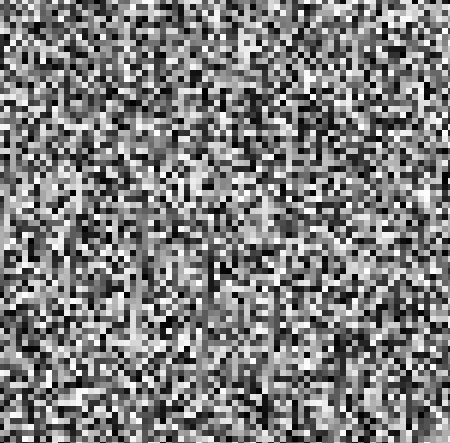
\includegraphics[scale=.49]{white_noise}
	
\includegraphics[scale=.49]{perlin_noise}
	\caption{White noise et Perlin noise}
	\label{fig:noises}
\end{figure}

Les fonctions les plus communes pour une génération de ce style sont de la famille des \textit{Gradient noise} (bruit de gradient) et \textit{Value noise} (bruit de valeur).
Un value noise est défini à partir d'un white noise de cette manière :

\begin{alignat*}{3}
	V(x,y) =f( &f(B(\floor{x},\floor{y}), &&B(\floor{x+1},\floor{y}), &&\fract{x}),\\
			&f(B(\floor{x},\floor{y+1}), &&B(\floor{x+1},\floor{y+1}), &&\fract{x}),\\
			&\fract{y})
\end{alignat*}

Ici $V$ est le value noise, $B$ est le white noise et $fract(x)$ est la partie fractionaire de $x$. $f$ dépend du value noise, c'est une fonction d'interpolation, la plus simple est l'interpolation linéaire\footnote{$lerp(a,b,x) = a+(b-a)*x$}.
L'idée est d'interpoler entre des valeurs complétement aléatoires selon une grille. Le value noise permet de générer des heightmaps très simplement, mais qui laissent à désirer. Aujourd'hui il a été très largement remplacé par le bruit de Perlin, qui est un cas spécifique de gradient noise.

La différence avec le value noise est qu'au lieu d'utiliser un white noise comme base, on génère à la place une grille de vecteurs unitaires et pour calculer les "$B(x,y)$" on calcule le produit scalaire du point $(x,y)$ à l'intérieur de sa cellule sur la grille avec les vecteurs unitaires :

\begin{align*}
	fx&=\floor{x} & a_{00}&=<(dx,dy), U_{fx,fy}>\\
	fy&=\floor{y} & a_{10}&=<(dx-1,dy), U_{fx+1,fy}>\\
	dx&=\fract{x} & a_{01}&=<(dx,1-dy), U_{fx,fy+1}>\\
	dy&=\fract{y} & a_{11}&=<(1-dx,1-dy), U_{fx+1,fy+1}>
\end{align*}
\begin{alignat*}{3}
	G(x,y) =f( &f(a_{00}, &&a_{01}, &&dx),\\
			&f(a_{10}, &&a_{11}, &&dx), dy)
\end{alignat*}

Dans son article\cite{perlinnoise}, Ken Perlin défini le \textit{Simple gradient noise} avec $f$ l'interpolation linéaire, et le bruit de perlin, avec $f$ la fonction $smoothstep$\footnote{$smoothstep(a,b,x) = 3x^2-2x^3$}.

Ces bruits sont bons pour un terrain simpliste, mais l'astuce de Ken Perlin est d'en cumuler plusieurs octaves. En jouant sur la fréquence et l'amplitude de chacune :
\begin{align*}
	Height(x,y) = \sum_{k=1}^{N}&Amplitude_k G(Frequency_k*(x,y))\\
	Amplitude_k &= Persistence^k\\ 
	Frequency_k &= Lacunarity^k
\end{align*}
Les paramètres qui nous restent à contrôler sont la persistance (le facteur de taille entre deux octaves), la lacunarité (le facteur de poids entre deux octaves) et le nombre d'octaves. Avec ceci on arrive à des cartes de hauteur assez réalistes, comme illustré en figure \ref{fig:layered_noise}.

\begin{figure}[h]
	\centering
	
\includegraphics[scale=.3]{perlin_1_octave}
	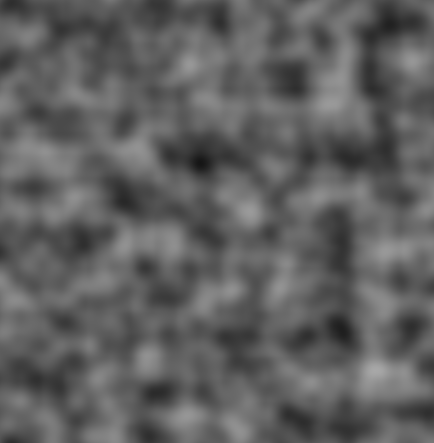
\includegraphics[scale=.3]{perlin_2_octaves}
	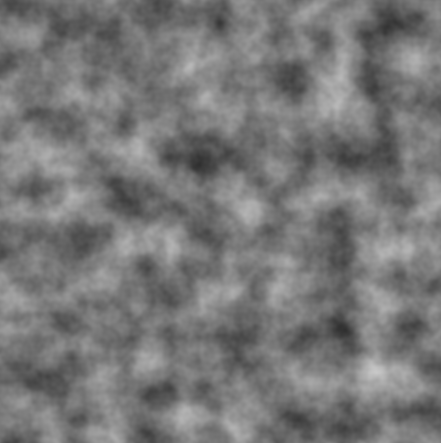
\includegraphics[scale=.3]{perlin_4_octaves}
	\caption{1, 2 et 4 octaves du Perlin noise}
	\label{fig:layered_noise}
\end{figure}

%%  TODO layered noise

\subsection{Erosion}

On peut rendre le bruit généré plus réaliste encore en appliquant des propriétés physiques naturelles, la première à laquelle on pense est l'érosion.

L'idée est de simuler un très grand nombre de gouttes d'eau qui dévallent les pentes en arrachant du sédiment du terrain et en la relachant en aval. L'algorithme que nous utiliserons est expliqué dans la thèse de Hans Theobald Beyer\cite{erosion}.
Dans le code cela consiste à calculer une suite de valeurs de gradient de la heightmap pour déplacer les gouttes selon la pente, et à chaque déplacement on calcule la quantité de sédiment à arracher ou déposer. Le seul bémol est que le dépot et l'érosion ne se font pas seulement à la position de la goutte, mais aussi aux alentours. Pour ne pas recalculer les différences à chaque étape de chaque goutte on fait le calcul en amont, qu'on stoque pendant toute la durée de l'algorithme. Cela peut poser certains problèmes de performance et de besoin en mémoire, l'espace mémoire nécessaire est en $O(n^2)$ avec la taille du terrain et le premier facteur du polynôme est très important.

\subsection{Structure du terrain}

On verra ensuite que penser à l'affichage du terrain avant de fixer sa structure est essentiel, avec une bonne structure l'affichage est plus simple et beaucoup plus performant. L'idée est que les données du terrain ne peuvent pas (ou peu) être modifiées pendant l'exécution mais qu'elle doivent pouvoir être segmentées pour n'en afficher qu'une partie.
Pour résoudre ce problème nous divisons le terrain en parcèles (\textit{chunks}). Chaque parcelle peut être générée et affichée indépendament des autres, seul sa position suffit à savoir ce qu'elle contient.
Avec cette division il est assez simple de faire un terrain qui se met à jour en fonction de la position du joueur, pour que les chunks proches soient toujours visible.

%% classes



\subsection{Variations}

%% liste des facteurs sur lesquels on peut jouer
%% génération de desert...




\section{Affichage 3D}

L'affichage représente la plus grosse partie du projet, on a beau avoir un terrain immense et avec des details très fins, s'il est impossible de l'afficher le tout n'a plus grand interet.

Nos contraintes principales seront de pouvoir afficher un très grand terrain, avec des performances qui permettent le déplacement en temps réel (60 images par secondes). Concrètement cela veut dire qu'afficher une image doit prendre moins de 16.6ms, ce qui peut être très difficile à respecter dans certains cas.

Avec ces considérations et notre experience passée commune, nous avons choisi d'utiliser OpenGL comme interface avec le gpu (carte graphique).

\subsection{OpenGL}

OpenGL est une spécification qui définie des points d'entrée d'une interface cpu-gpu. Pour utiliser OpenGL nous avons besoin d'une librairie dépendante du langage de programmation ; en c++ nous utiliserons glad. Nous aurons aussi besoin de librairies pour la gestion de la fenêtre de l'application et l'interface utilisateur, nous utiliserons glfw et ImGui.

\paragraph{}
OpenGL fonctionne comme une \textit{state machine}. Chaque fonction modifie l'état interne du gpu et certaines lances des commandes à exécuter comme l'affichage de formes géométriques.
Il est important de mentionner que les gpu modernes ne savent pas afficher autre chose que des triangles et des lignes, pour afficher un rectangle on devra se contenter de dessiner deux triangles.

\subsection{Shaders}

Les \textit{shaders} sont des programmes qui tournent sur le gpu plutot que sur le cpu. Nous utiliserons extensivement deux types de shaders pour l'affichage : le \textit{vertex shader} qui s'execute pour chaque sommet des triangles affichés ; et le \textit{fragment shader} qui s'execute pour chaque pixel couvert par le triangle. Des shaders classiques ressemblent à ceci :
%% TODO vertex shader

Un dernier type de shader que nous utiliserons est le \textit{compute shader}, qui ne sert pas à l'affichage mais permet de faire des calculs massivement parrallèles sur le gpu. Il nous sera utile pour gagner en performance.

\paragraph{}
Avec ces éléments définis on peut faire un schéma de la "pipeline OpenGL" :
%% TODO schema pipeline


\subsection{Caméras et mathématiques}

\subsection{Ombres}

Nous avons implémenté deux types d'ombre : les ombres d'ambiance et les ombres portées. Les deux se combinent très facilement dans le fragment shader utilisé pour le terrain.
\subsubsection{Ombre d'ambiance}
Une ombre d'ambiance est l'obsurcissement des surfaces qui ne sont pas dirigées vers le soleil. Mathématiquement cela se calcule très bien à partir des normales du terrain, pour chaque pixel on calcule ce que reçoit le pixel :
$$ S_{ambiance}=max(0, \vec{N}\cdot \vec{D}) $$
Avec $\vec{N}$ la normale du terrain à la position du pixel, $\vec{D}$ la direction des rayons su soleil comme illustré dans la figure \ref{fig:ambiant_shadows_schema}.

\begin{figure}[h]
	\centering
	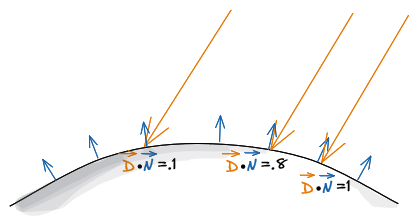
\includegraphics[scale=.49]{ombres_ambiantes}
	\caption{Schéma du fonctionnement des ombres ambiantes}
	\label{fig:ambiant_shadows_schema}
\end{figure}

\subsubsection{Ombre portées}
Le calcul des ombres portées et autrement plus compliqué, et se divise en plusieurs étapes
\begin{enumerate}
\itemsep-.5em
\item positionner le soleil pour qu'il éclaire le moins possible
\item afficher la scène "depuis le point de vue du soleil"
\item afficher la scène normalement, en tenant compte de la distance des objets au soleil
\end{enumerate}

\begin{figure}[h]
	\centering
	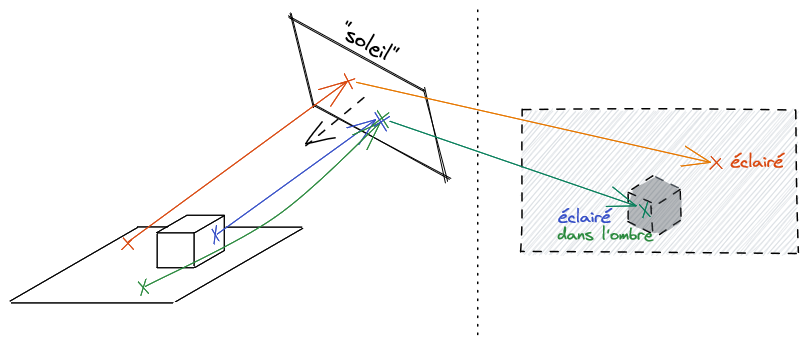
\includegraphics[scale=.49]{ombres}
	\caption{Schéma du fonctionnement des ombres portées}
	\label{fig:shadows_schema}
\end{figure}

L'idée est de calculer la distance des pixels au soleil et de vérifier que cette distance est bien la plus petite à la position du pixel du point de vue du soleil (en bleu et orange sur la figure \ref{fig:shadows_schema}), si ce n'est pas le cas cela signifie qu'un autre objet est plus proche du soleil et donc qu'il projète une ombre sur le pixel (en vert sur le schéma).

\paragraph{}
Le positionnement se fait en listant les objets qui doivent recevoir et pouvoir projeter des ombres. Tout les éléments qui ne sont pas dans le champ de vue du joueur n'ont pas à être éclairés mais ceux qui peuvent projeter des ombres sur des objets visibles doivent être pris en compte.
%% TODO maths?
%% TODO screen du positionnement de la sun camera
\paragraph{}
L'affichage de la scène depuis le point de vue du soleil utilise une caméra orthographique car tous les rayons sont perpendiculaires. La distance la plus faible est enregistrée pour chaque pixel et est utilisée ensuite. La distance enregistrée ainsi est normalisée (linéarisée dans $[0,1]$) par OpenGL. La texture qui contient ces distances est appellée \textit{depth map}(\textit{carte de profondeur}).

\subsubsection{Algorithme final}

Après que la depth map ai été calculée, on arrive à un algorithme de ce type pour déterminer la quantité de soleil que reçoit chaque pixel.
\begin{algorithm}
\caption{Calcul des ombres par pixel}
\begin{algorithmic}
\State $P_s \gets \text{... matrice de projection monde$\rightarrow$depth map}$
\State $DM \gets \text{... depth map 2D}$
\State $D \gets \text{... direction des rayons du soleil}$
\\
\State $p \gets \text{...  position 3D du pixel}$
\State $n \gets \text{... normale 3D à la position du pixel}$
\\
\State $S_{ambiant} \gets max(0, n\cdot D)$
\State $u \gets P_s\times p$
\State $d_{pixel} \gets u.z$
\State $d_{nearest} \gets DM(u.xy)\times(z_{far}-z_{near})+z_{near}$
\State $S_{casted} \gets smoothstep(-\epsilon, 0, d_{pixel}-d_{nearest})$
\State $Q \gets S_{ambiant}*S_{casted}$
\\
\State $PixelColor\gets mix(SunDarkColor, SunLightColor, max(.1, Q\times SunStrength))$
\end{algorithmic}
\end{algorithm}

On préfère utiliser la fonction $smoothstep$ et utiliser $\epsilon$ plutôt que de mettre $S_{casted}$ à $0$ ou $1$ pour éviter le crénelage du aux erreurs d'arrondis.

%% TODO screen des ombres

\subsection{Instanced rendering}
\label{section:instanced_rendering}

En plus du terrain en lui même, nous avons choisi d'afficher quelques objets en plus. Et par "quelques" il faut entendre plusieurs millions. Nous nous sommes donné le but d'afficher des brins d'herbe, nous reviendrons sur les algorithmes d'optimisation mis en place mais avant de pouvoir en discuter il est important de comprendre \textit{comment} OpenGL gère l'affichage.
\paragraph{}
Pour afficher un objet simple (un cube par exemple) il nous faut 4 structures de données sur le gpu : un \textit{Vertex Buffer}, qui contient les données de chaque sommet du cube ; un \textit{Index Buffer}, qui définit les triangles à partir des sommets ; un shader et un \textit{Vertex Array} que nous passerons sous silence car ils n'influencent pas les données.

Une manière très naïve d'afficher un très grand nombre d'éléments est de construire un Vertex Buffer (VB) et un Index Buffer (IB) par objet. Le soucis est qu'à l'affichage il nous faudra changer le contexte OpenGL (modifier les VB/IB actifs) pour chaque élément, ce qui ralentit considérablement le tout\footnote{Le vrai problème vient du nombre d'appels à des fonctions d'affichage, il est possible d'afficher beaucoups d'éléments d'un coup mais seulement si le contexte n'a pas à changer}.
Si les objets sont identiques on peut n'utilser qu'un seul IB, mais ce n'est pas suffisant.

\paragraph{}
Une manière déjà plus intéressante est de construire un unique VB qui contient tout les sommets de tout les éléments et un IB qui contient les triangles constitués de ces sommets, cela améliore déjà considérablement les performances. Cette méthode est appellée \textit{batch rendering}.
Cette méthode possède cependant un désavantage majeur, il est quasiment impossible de n'afficher qu'une partie des éléments. Pour le terrain par exemple nous n'affichons que les chunks visibles par la caméra, le batch rendering n'est donc pas adapté. On préferera faire des chunks de grande taille pour diminuer le nombre de changement de contextes même si cela diminue l'éfficacité de n'afficher que les chunks visibles.

\paragraph{}
Dans notre cas on peut encore faire mieux, tout nos éléments sont identiques mis à part leurs position dans le monde, on peut donc utiliser un seul VB et IB qui contiennent les données d'un unique brin d'herbe et le dessiner autant de fois que nécessaire à des positions différentes. Mais pour ne pas avoir à modifier le contexte OpenGL il faut que ces données d'instances soient présentes sur le gpu. On créé donc un \textit{instance buffer} qui contient la position de chaque brin d'herbe. Cette méthode s'appelle l'\textit{instanced rendering}.

\begin{figure}[h]
	\centering
	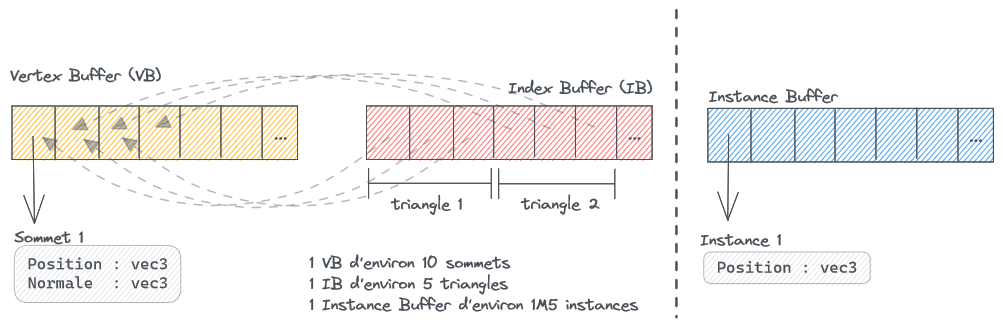
\includegraphics[scale=.4]{grass_vbibib}
	\caption{Structures présentes sur le gpu en instanced rendering}
	\label{fig:grass_vbibib}
\end{figure}

\subsubsection{Profilage}
Avec l'instanced rendering on peut afficher plusieurs centaines de milliers de triangles sans trop impacter les performances, mais ce n'est pas suffistant pour les quelques millions que nous nous sommes fixé, nous reviendrons sur les deux optimisations majeures dans la section \ref{section:grass_rendering}.
\paragraph{}
 Pour vérifier que notre implémentation est déjà meilleure que la naïve on peut comparer le temps mit avec les deux méthodes. Le profilage doit se faire avec des outils adaptés et non pas depuis C++ car le gpu et le cpu ont des fils d'execution très différents.

%% TODO screen des benchmarks

\subsection{Effets spéciaux}

\subsubsection{} %% ...




\section{Algorithmes spécifiques}

%% algos qu'on a développé avec plus ou moins de sources (plutot moins que plus)

\subsection{Affichage de l'herbe}
\label{section:grass_rendering}

Nous avons déjà abordé l'instanced rendering dans la section \ref{section:instanced_rendering}. Néanmoins pour afficher plusieurs millions de brins d'herbe d'autres techniques sont nécessaires. On peut déjà imaginer afficher deux modèles différents, un en haute résolution (7 ou 8 triangles) et un en basse résolution (1 triangle) qui sera utilisé pour les brins d'herbes loin de la caméra. On peut aussi n'afficher que les brins d'herbe visible ; on ne peut pas replacer les brins d'herbe en permanence car l'envoi de données du cpu au gpu est lent, mais on peut dire au gpu de filtrer les brins d'herbe qui ne sont pas visible pour qu'ils ne fassent pas partie de la prochaine commande d'affichage.

\paragraph{}
La méthode que nous utiliserons pour filtrer les brins d'herbe visibles est inspirée de la vidéo d'Acerola\cite{grass_rendering}. L'idée est de maintenir deux instance buffers : le complet, qui contient tous les brins d'herbe et n'est mit à jours que lorsque le joueur se déplace beaucoup pour qu'il soit toujours au milieu de la zone couverte de brins d'herbe ; et un deuxième qui contient seulement les brins d'herbe visible et est mit à jours à chaque frame. L'algorithme s'appelle le scan and compact, une version parrallèle est l'algorithme \ref{alg:scan_and_compact}.

\begin{algorithm}
\caption{Scan and compact}\label{alg:scan_and_compact}
\begin{algorithmic}
\State $I \gets \text{... instance buffer complet}$
\State $N \gets |I|$
\\
\State $V \gets \{0\}^N$ \Comment{Vote buffer}
\State $S \gets \{0\}^N$ \Comment{Scan buffer}
\State $B \gets \{nil\}^N$ \Comment{Compact buffer}
\State $M \gets 0$ \Comment{nombre total d'instances visibles}
\\
\ParFor{$i\gets 1, N$}
	\State $V_i \gets vote(I_i)$ \Comment{Vote, $V_i$ vaudra 1 ssi l'instance est visible}
\EndParFor
\State $S,M\gets Scan(V)$\Comment{Scan du vote buffer, cad $S_i\gets\sum_{k=1}^i V_k$}
\ParFor{$i\gets 1,N$}
	\If{$V_i=1$}
		\State $B_{S_i}\gets I_i$\Comment{Compact, les instances visibles remplissent $B$}
	\EndIf
\EndParFor
\end{algorithmic}
\end{algorithm}

L'avantage du gpu est que les calculs sont massivement parrallélisables. Nous avions vu l'algorithme de scan l'année dernière en CUDA en cours. Nous n'avons pas pu récuperer l'algorithme car OpenGL permet seulement de synchroniser les threads d'un groupe et pas les groupes entre eux et nous sommes limités en nombre de threads/groupes. En terme moins technique cela signifie que l'algorithme de scan doit se diviser en trois parties parrallèles.

\paragraph{}
En étant limité à $N=1024$ threads/groupe et $G=1024$ groupes, l'algorithme que nous proposons est limité à $G\times N=1'048'576$ brins d'herbe, et peut facilement être étendu à $G\times N^M$ en répétant $M$ fois les étapes 2 puis 3.

\begin{tabular}{|l|l|l|}
	\hline
	 & $\makecell{Threads\times\\ Groupes}$ & action\\
	\hline
	1. scan/block & $N\times  G$ & \makecell[l]{On scanne sur $V_i$ chaque block de $N$ brins\\ d'herbe, le total de chaque block est\\ stoqué dans $A_i$}\\
	\hline
	2. scan/group & $G\times 1$ & \makecell[l]{On scanne sur $A_i$ les sommes de chaque\\ block, le total est stoqué dans $M$}\\
	\hline
	3. accumulation & $N\times G$ & \makecell[l]{On ajoute à chaque valeur de chaque block\\ (les $V_i$) la somme des sommes des\\ blocks précédents (les nouveaux $A_i$)}\\
	\hline
\end{tabular}

\paragraph{}
On peut ensuite afficher $M$ brins d'herbe.

%% TODO screen de l'herbe

\subsection{Eau}



\section{Résultats}

%% screens


%% \section{Performances} %% si on a encore la foi d'écrire

\begin{thebibliography}{9}
\bibitem{perlinnoise}
Perlin, Ken. "Making Noise"

\bibitem{erosion}
Hans Theobald Beyer. "Implementation of a method for hydraulic erosion"

\bibitem{grass_rendering}
Acerola, "What I Did To Optimize My Game's Grass", \url{https://youtu.be/PNvlqsXdQic}
\end{thebibliography}

\listoffigures

\end{document}
